\section{Entorno de Desarrollo Local}

Para garantizar la reproducibilidad del proyecto, en esta sección se descibirá el entrono de desarrollo en el que se ha realizado y el acceso al repositorio con el código fuente.

\subsection{Tecnologías y Versiones}

El proyecto se ha desarrollado en un entorno \textbf{Windows 10}, aunque esto no influye en la compatibilidad, ya que todas las tecnologías utilizadas son multiplataforma, lo cual permite realizar el desarrollo en cualquier sistema operativo sin restricciones. En la tabla \ref{tab:dependencias_versiones} se presentan las tecnologías principales empleadas en el proyecto junto con sus versiones correspondientes.

\begin{table}[htbp]
    \centering
    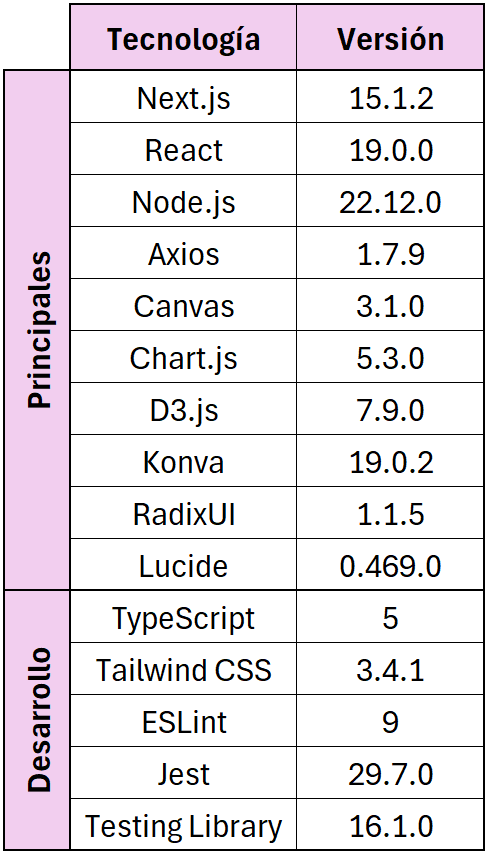
\includegraphics[width=0.37\textwidth]{figures/dependencias_versiones.png}
    \captionsetup{skip=5pt}
    \caption{Dependencias usadas en el desarrollo, junto con sus versiones.}
    \label{tab:dependencias_versiones}
\end{table}

Cabe destacar que el gestor de paquetes utilizado en el proyecto ha sido \textbf{\texttt{pnpm} (\textit{Performant Node Package Manager})}, en lugar de \texttt{npm} (\textit{Node Package Manager}) o \texttt{yarn} (\textit{Yet Another Resource Negotiator}). La elección de \texttt{pnpm} se debe a sus mejoras en la gestión de dependencias y optimización del uso del espacio de almacenamiento. A diferencia de \texttt{npm}, \texttt{pnpm} utiliza un sistema de enlaces en lugar de duplicar archivos en cada proyecto, lo que reduce significativamente el consumo de espacio. Además, \texttt{pnpm} es completamente compatible con los paquetes del registro de \texttt{npm}, lo que garantiza su interoperabilidad con la mayoría de los ecosistemas de desarrollo basados en \textit{Node.js}.

\subsection{Instalación y Configuración del Proyecto}

El proyecto se encuentra alojado en un repositorio de \textit{GitHub}\footnote{Repositorio del proyecto: \href{https://github.com/jonortega/tfg-app-spotify}{https://github.com/jonortega/tfg-app-spotify}} para evitar pérdidas y tener disponibilidad completa al código. Para ejecutarlo localmente, además de haber instalado \textit{Node.js}, hay que clonar el respositorio, acceder a la carpeta y ejecutar los comandos de instalación y ejecución. A continuación, se muestran los comandos necesarios para realizar estos pasos:

\begin{ifalgorithm}[H]
    \begin{lstlisting}[language=bash]
    # Clonar el repositorio
    git clone https://github.com/jonortega/tfg-app-spotify.git
    
    # Acceder al directorio del proyecto
    cd tfg-app-spotify
    
    # Instalar dependencias
    pnpm install
    
    # Ejecutar el servidor de desarrollo
    pnpm run dev
    \end{lstlisting}
    \caption{Comandos de instalación y ejecución inicial del proyecto.}
    \label{alg:instalacion_proyecto}
\end{ifalgorithm}

Tras estos pasos, la página web estará accesible en \texttt{localhost:3000}. Es encesario agregar un fichero de variables de entorno \texttt{.env.local}, ya que, por seguridad, no se registra en el sistema de control de versiones. El contenido de dicho fichero se muestra en el \hyperref[ch:anexoC]{Anexo C} (algoritmo \ref{alg:variables_entorno}).

Dos de las variables de entorno necesarias para poder tratar con la API de \textit{Spotify}, son el \textbf{Client ID} y el \textbf{Client Secret}. Estos dos valores se obtienen al realizar el registro de la aplicación en la plataforma de desarrollo de \textit{Spotify}. En la siguiente sección, se explicará cómo realizar este registro y dónde obtener dichas variables.

\newpage

\section{Registro de la Aplicación en Spotify}

Para poder obtener datos de la Web API de \textit{Spotify}, es necesario registra la aplicación en su plataforma de desarrollo\footnote{Spotify for Developers: \href{https://developer.spotify.com/}{https://developer.spotify.com/}}. Tras inciar con una cuenta, se nos presentará un panel donde podremos crear una nueva app. \textit{Spotify} pedirá algunos datos (figura \ref{fig:create_app}), que tendremos que rellenar. Los campos como \textit{Redirect URIs} pueden ser modificados posteriormente, ya que tendremos que actualizarlo con el dominio indicado tras el despliegue de la aplicación.

\begin{figure}[H]
    \centering
    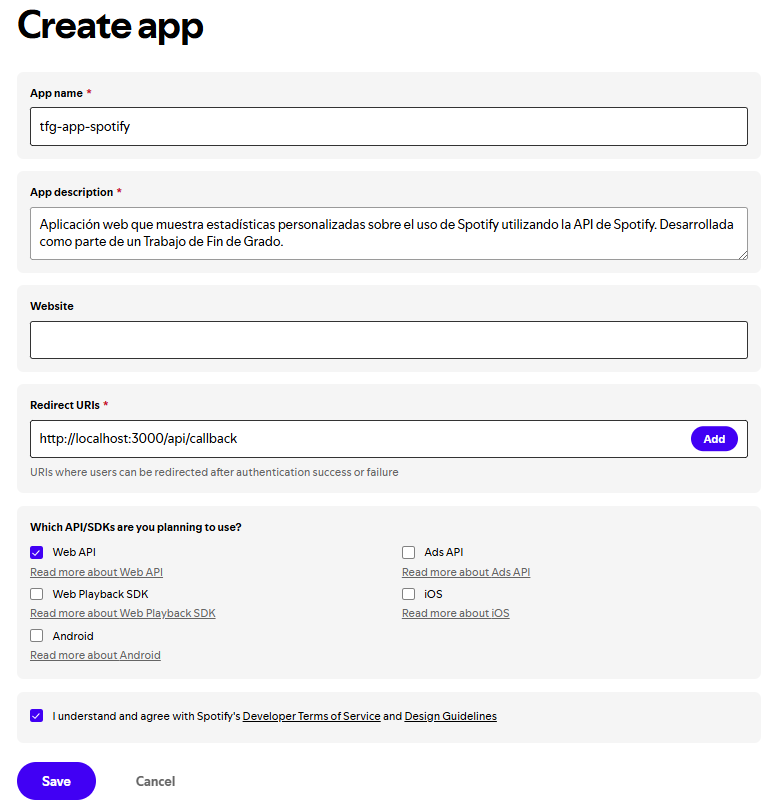
\includegraphics[width=0.65\textwidth]{figures/registro_spotify/create_app.png}
    \caption{Panel de creación de app en la plataforma de \textit{Spotify}.}
    \label{fig:create_app}
\end{figure}

Al aceptar los términos y crear la app, tendremos acceso al \textit{Client ID} y \textit{Client Secret}. Estos se encuentran en los ajustes (\textit{settings}) y tendremos que expandir el panel para poder ver los dos valores (figura \ref{fig:client_id_secret}).

\begin{figure}[H]
    \centering
    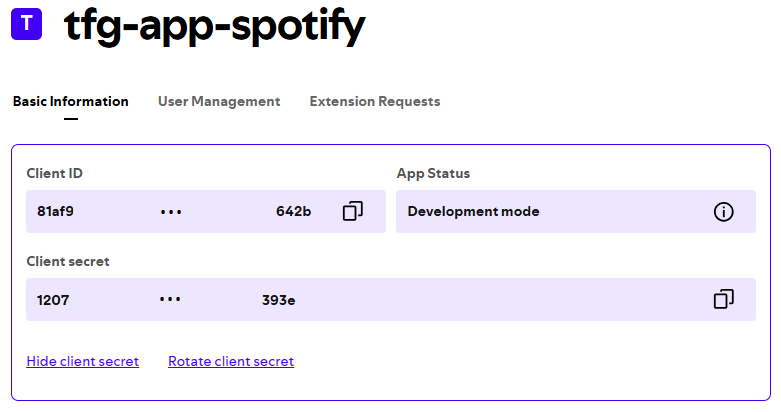
\includegraphics[width=0.65\textwidth]{figures/registro_spotify/client_id_secret.png}
    \caption{Panel de ajustes con el \textit{Client ID} y el \textit{Client Secret}.}
    \label{fig:client_id_secret}
\end{figure}

En el caso en el que el \textit{Client Secret} haya sido comprometido, es posible generar uno nuevo, anulando el anterior y evitando tener que desechar la aplicación registrada. También se muestra un campo llamado \textit{App Status} con el valor \textbf{Development Mode}. Esto significa que la aplicación registrada está en ``desarrollo'', por lo que existen las siguientes restricciones:

\begin{itemize}
    \item Un máximo de 25 usuarios (cuentas verificadas de \textit{Spotify}) pueden usar la aplicación.
    \item Cada usuario tiene que estar registrado en una lista de permitidos (\textit{allowlist}) de la plataforma.
\end{itemize}

Es posible eliminar estas restricciones, enviando una solicitud a \textit{Spotify} para cambiar el estado de \textit{Development Mode} a \textbf{Extended Quota Mode}. En el caso de que sea aceptada, se elimina cualquier restricción sobre el número de usuarios permitidos y no será necesario registrarlos anteriormente, además de ampliar el umbral de la tasa de peticiones (\textit{rate limit}). En este trabajo \textbf{no se va a realizar dicha solicitud}, por lo que tendremos que acogernos a las limitaciones impuestas en el modo de desarrollo. Esto requiere que se registren las cuentas de usuarios que vayan a probar la aplicación en la pestaña de gestión de usuarios (figura \ref{fig:user_management}).

\begin{figure}[H]
    \centering
    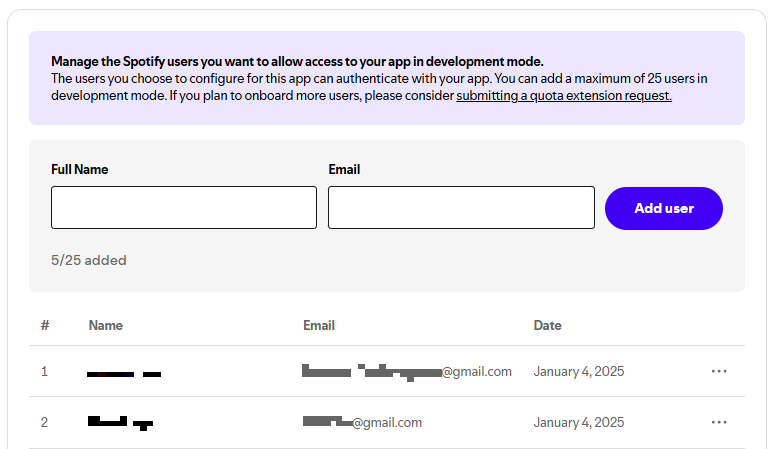
\includegraphics[width=0.75\textwidth]{figures/registro_spotify/user_management.png}
    \caption{Panel de gestión de usuarios que tienen acceso a la aplicación.}
    \label{fig:user_management}
\end{figure}

Con estos pasos, se habrá realizado correctamente el registro de la aplicación y obtención del \textit{Client ID/Secret}, imprescindibles para la comunicación con la API de \textit{Spotify}. En la plataforma de desarrollo, además, tenemos accesible un panel para poder monitorear la actividad de la aplicación (\hyperref[ch:anexoC]{Anexo C}, figura \ref{fig:dashboard_spotify}).

\section{Ciclo de Desarrollo}

El ciclo de desarrollo del proyecto ha seguido un enfoque híbrido entre los modelos \textbf{incremental} e \textbf{iterativo}. En concreto, se ha construido en tres incrementos, realizados en diferentes puntos del proyecto. En cada uno, se han añadido más funcionalidades (incremental) y refinando las ya existentes (iterativo). A continuación se describe cada incremento con más detalle.

\subsection*{Incremento I: Prototipado Rápido}

Durante la fase inical de adquisición de competencias, se desarrolló un prototipo rápido para validar la viabilidad técnica del proyecto. No se buscaba crear la base desde donde seguir trabajando una vez inicase el desarrollo formal; si no que, utilizando herramientas más simples, se quería obtener una idea preliminar de cómo se podrían implementar las funcionalidades principales. No se utilizaron las tecnologías finales del desarrollo, por lo que gran parte del código implementado no fue reutilizado.

En este prototipo se implementaron las siguientes funcionalidades, en diferentes grados de completado:
\setlength{\itemsep}{0pt}
\begin{itemize}
    \item Inicio de sesión de un usuario y obtención de los tokens.
    \item Renovación del \texttt{access\_token} mediante el \texttt{refresh\_token}.
    \item Obtener los \textit{top items} del usuario.
    \item Obtener las canciones favoritas del usuario.
    \item Obtener los \textit{track features} (\textbf{no implementado en el producto final}).
    \item Prototipos de las estadísticas:
          \begin{itemize}
              \item \textit{Hall Of fame}
              \item \textit{Huella Del Día}
              \item \textit{La Bitácora}
          \end{itemize}
\end{itemize}

\subsection*{Incremento II: Producto Mínimo Viable (PMV)}

Una vez terminada la planificación del proyecto, se dio comienzo a una primera implementación del sistema, desarrollando una base de código que formaría parte del producto final. En esta fase, se utilizaron todas las tecnologías finales seleccionadas para el desarrollo, incluyendo \textit{Next.js}, \textit{React}, TypeScript y \textit{Tailwind CSS}.

Durante este incremento, se completaron las siguientes partes fundamentales del sistema:

\setlength{\itemsep}{0pt}
\begin{itemize}
    \item Estructura completa de páginas de la aplicación web.
    \item Implementación de los endpoints mediante \textit{Route Handlers}.
    \item Inicio de sesión y cierre de sesión seguros.
    \item Gestión segura de los tokens.
    \item Implementación de las estadísticas básicas \textit{Top Tracks}, \textit{Top Artists}, \textit{Top Genres} y \textit{Recently Played}.
    \item Desarrollo inicial de las seis estadísticas avanzadas finales en un estado funcional básico.
\end{itemize}

Si bien estas estadísticas se implementaron de manera inicial y sin refinamientos, su propósito principal fue definir la interacción entre el frontend y el backend, establecer los tipos de datos y endpoints exactos requeridos, y detectar posibles problemas en la presentación de la información. Asimismo, esta fase permitió identificar la necesidad de herramientas adicionales, como bibliotecas de gráficos, en caso de que las opciones disponibles no fueran suficientes.

En términos generales, este incremento sirvió para caracterizar con mayor precisión el alcance del proyecto y definir con claridad los aspectos que deberían considerarse en las siguientes etapas de análisis y diseño. A diferencia del prototipo inicial, gran parte del código desarrollado en esta iteración se integró directamente en la versión final del sistema.

\subsection*{Incremento III: Producto Final}

Finalmente, en el último incremento se completaron todas las funcionalidades secundarias pendientes, junto con una serie de optimizaciones de rendimiento, ajustes en las estadísticas avanzadas y mejoras en la interfaz y experiencia de usuario. Esta fase marcó la consolidación del sistema y la preparación del código para su despliegue.

Las principales funcionalidades implementadas y correcciones realizadas fueron:

\setlength{\itemsep}{0pt}
\begin{itemize}
    \item Posibilidad de cambiar el rango temporal en los módulos \textit{Top Tracks}, \textit{Top Artists} y \textit{Top Genres}.
    \item Implementación de la funcionalidad para crear playlists en \textit{Hall Of Fame}.
    \item Desarrollo de la estadística \textit{Tus Décadas} utilizando la librería \textit{Konva} para una mayor optimización.
    \item Mejora en la presentación y rendimiento de la estadística \textit{Índice de Interferencia} con \textit{D3.js}.
    \item Corrección en la estructura de datos enviada desde el backend a la estadística \textit{La Bitácora}.
    \item Implementación de la ventana informativa sobre la \textit{Política de Privacidad}.
    \item Reemplazo de la implementación manual de la ventana modal de las estadísticas por la librería \textit{Radix UI}.
    \item Creación de componentes de carga (\textit{loading components}).
    \item Gestión de errores encontrados al probar con diferentes cuentas de usuario.
    \item Desarrollo de una pantalla de carga específica para las estadísticas avanzadas.
    \item Refactorización del código para crear funciones reutilizables, como en la obtención de datos (\textit{fetch}), facilitando la gestión de los componentes.
    \item Preparación del código para su despliegue en \textit{Vercel}, especialmente la gestión de variables de entorno.
\end{itemize}

Este último incremento permitió completar todas las funcionalidades planeadas y refinar el sistema en su conjunto. Además de las mejoras implementadas, se documentaron posibles optimizaciones futuras, aunque, dentro del alcance definido para el proyecto, la aplicación alcanzó un estado final funcional y estable.

Cabe destacar que las listas de funcionalidades y mejoras descritas en cada incremento no son exhaustivas, sino que recogen las implementaciones y cambios más relevantes realizados durante el desarrollo. A lo largo del proceso, se llevaron a cabo numerosas correcciones, ajustes e implementaciones adicionales que no se han detallado en su totalidad. No obstante, estas listas permiten ofrecer una visión general de los aspectos más significativos de cada incremento en el desarrollo del proyecto.

\section{Gestión Segura de los Tokens}

Antes de poder interactuar con la API de \textit{Spotify}, es fundamental obtener y poder gestionar correctamente los tokens de autenticación que, como se ha descrito anteriormente en la sección de \nameref{sec:diseno_seguridad}, se han decidido tomar ciertas medidas. En dicha sección, se abordó el tema desde una perspectiva de diseño y un nivel más alto de abstracción, mientras que en esta, se profundizará en los aspectos más técnicos.

En primer lugar, el \textit{Client ID} y \textit{Client Secret} se alamacenan en el servidor, en respectivas variables de entorno, y solo se acceden desde el objeto \texttt{process.env}. Estos tokens nunca son enviados al cliente y se usan en casos concretos, como en el inicio de sesión de un nuevo usuario o la renovación del \texttt{access\_token}.

Por otro lado, la gestión del propio \texttt{access\_token} requiere más atención. Se evaluaron varias opciones, pero finalmente se decidió en hacer uso de las \textbf{cookies}. Esto se debe a que, de esta manera, no era necesario implementar un sistema de almacenamiento en el servidor (manual o mediante herramientas como \textit{Redis}) para guardar los \texttt{access\_token} de los diferentes usuarios y asociarlos a un identificador único. El propio \texttt{access\_token} hace de identificador de cada usuario, por lo que el servidor solo tiene que hacer uso del token recibido mediante las cookies agregadas en la petición.

No obstante, es importante utilizar los sistemas de seguridad que las propias cookies ofrecen, para limitar cualquier tipo de uso malintencionado del token. Existen ciertas opciones (\textit{flags}) de configuración que se han establecido:

\setlength{\itemsep}{0pt}
\begin{itemize}
    \item \textbf{httpOnly}: \textbf{Impide que el token sea accesible mediante JavaScript en el navegador}, protegiéndolo contra ataques de tipo \textit{Cross-Site Scripting} (XSS).
    \item \textbf{secure}: Se asegura de que las cookies \textbf{solo sean enviadas a través de conexiones HTTPS}, protegiéndolas contra ataques de interceptación de tráfico (\textit{Man-in-the-Middle}, MITM). Esta opción solo se habilita cuando la aplicación se ejecuta en un entorno de producción.
    \item \textbf{maxAge}: Define el tiempo de \textbf{expiración de las cookies}. El \texttt{access\_token} tiene una validez de una hora, mientras que el \texttt{refresh\_token} se mantiene activo durante 24 horas, permitiendo la renovación del token de acceso sin necesidad de solicitar credenciales nuevamente.
\end{itemize}

Estableciendo de esta manera el \texttt{access\_token} y el \texttt{refresh\_token} en las cookies y enviándolas en la respuesta al cliente, se mantiene la posibilidad de que cada usuario envíe su propio token como identificador, pero manteniendo la seguridad frente a ataques comunes. También se debe mencionar que, por el hecho de haber habilitado el \textit{flag} \texttt{httpOnly}, \textbf{ningún componente de cliente puede realizar peticiones directamente desde el neavegador}. Todas las peticiones de datos a la API de \textit{Spotify} deben de ser realizadas a tráves del backend seguro.

\subsection*{Implicaciones de la Decisión del uso de las Cookies}

El uso de las cookies como forma de almacenamiento del identificador también requiere el conocimiento del alcance efectivo de este sistema, que permite identificar posibles limitaciones que este método impone. Las cookies son compartidas entre todas las pestañas y ventanas del mismo navegador mientras se mantengan dentro del mismo dominio, lo que permite que la autenticación y la sesión del usuario se mantengan consistentes en diferentes contextos de navegación. Estas no se comparten entre distintos navegadores, ya que cada uno gestiona su propio almacenamiento de cookies.

Sin embargo, este sistema es \textbf{vulnerable si un atacante tiene acceso físico a la máquina} del usuario con la sesión abierta. A través del panel de desarrollador del navegador, el atacante podría visualizar directamente los valores de los tokens almacenados en las cookies. Aunque este método de almacenamiento impide el acceso mediante sistemas automatizados, un atacante con acceso manual al dispositivo podría extraer y utilizar estos valores.

Una posible medida de mitigación sería cifrar los tokens antes de almacenarlos en las cookies. No obstante, \textbf{se ha decidido no implementar esta solución} debido a varias razones: en primer lugar, por las limitaciones de alcance del proyecto; en segundo lugar, por la carga computacional adicional que supondría para el servidor el proceso de cifrado y descifrado en cada solicitud del usuario; y, finalmente, porque se considera que la probabilidad de que un atacante tenga acceso físico a una sesión abierta del usuario es extremadamente baja, lo que no justifica la implementación de este mecanismo en un sistema de estas características.

\section{Implementación del Frontend}

En los siguientes apartados, se describe el flujo de datos y la estructura utilizada para cargar y renderizar las estadísticas dentro de la aplicación, así como los aspectos más relevantes, como el paso de información entre componentes y la actualización de estados en componentes externos.

\subsection{React Hooks}

Para comprender mejor la implementación de los componentes, se considera importante hacer un inciso para introducir un concepto muy importante en \textit{React}: los \textbf{hooks}. Estos son funciones especiales proporcionadas por la API de \textit{React} que permiten a un componente funcional ``engancharse'' al estado y al ciclo de vida del mismo, sin necesidad de utilizar clases, y su uso está limitado a los componentes de cliente.

En el desarrollo de esta aplicación, se han empleado diversos \textit{hooks}. A continuación, se describen los principales \textit{hooks} utilizados y su aplicación en el proyecto:

\begin{itemize}
    \item \textbf{\texttt{useState}}: Permite manejar el \textbf{estado local} dentro de los componentes. Es uno de los \textit{hooks} más utilizados en desarrollos de \textit{React}.

    \item \textbf{\texttt{useEffect}}: Se emplea para \textbf{gestionar efectos secundarios} dentro de los componentes, como la obtención de datos o la suscripción a eventos. En este caso, se ha utilizado para realizar llamadas a los \textit{Route Handlers} del backend y poder obtener los datos en el cliente.

    \item \textbf{\texttt{useRef}}: Facilita el acceso a elementos del DOM y la \textbf{persistencia de valores entre renderizados} sin provocar re-renderizaciones innecesarias. Se ha utilizado en algunos componentes para manejar referencias a elementos gráficos, como un \textit{canvas} o contenedores, permitiendo obtener sus dimensiones y ajustar los renderizados en consecuencia.
\end{itemize}

Además, se ha desarrollado un \textbf{hook personalizado} denominado \textbf{\texttt{useFetch}}, el cual encapsula la lógica de obtención de datos de la API dentro de un \texttt{useEffect}. Este \textit{hook} es utilizado por los componentes de cliente para realizar peticiones de manera reutilizable. Se incluye el código detallado en el anexo, en el algoritmo \ref{alg:use_fetch}.

Cabe destacar que \textbf{Next.js} incorpora el modo de desarrollo \textbf{StrictMode}, el cual ejecuta los efectos definidos en \texttt{useEffect} dos veces consecutivas. Esto significa que, cuando un efecto se dispara, se ejecuta y se detiene inmediatamente para volver a ejecutarse desde cero. Este comportamiento permite detectar efectos mal programados y verificar si se están limpiando correctamente, evitando posibles errores que puedan aparecer en producción. Para gestionar correctamente este comportamiento, es necesario definir una \textbf{función de limpieza} dentro del \texttt{return} de \texttt{useEffect}. En este proyecto, la principal aplicación de este mecanismo ha sido la cancelación de las peticiones al backend. Para ello, se ha empleado la señal de aborto (\texttt{AbortController}) de la API \texttt{fetch}, la cual permite interrumpir una solicitud incluso si ya ha sido iniciada.

\subsection{Estadísticas Básicas (Home)}

Las estadísticas básicas se encuentran en la pantalla de inicio (\textit{Home}) y se implementan como \textbf{componentes de servidor}. Dado que estos componentes no se ejecutan en el navegador, pueden realizar peticiones al backend obteniendo directamente el \texttt{access\_token} desde las cookies, sin necesidad de gestionarlo manualmente en el cliente. Por otro lado, el selector de rango temporal (\textbf{TimeRangeSelector}) permite modificar la visualización de las estadísticas en función de tres intervalos: \texttt{short\_term}, \texttt{medium\_term} y \texttt{long\_term}, siendo \texttt{short\_term} la opción por defecto. Este selector es un \textbf{componente de cliente} que detecta cambios en su estado y, al modificarse, \underline{realiza una nueva petición al endpoint \texttt{/home}} con el \texttt{time\_range} seleccionado como parámetro en la URL.

El componente \textbf{Home} recibe este parámetro y lo propaga a los componentes de estadísticas mediante \textbf{props} (ver código en el anexo, algoritmo \ref{alg:home_component}), propiedades (o parámetros) de los componentes. Cuando se detecta un cambio en los datos, los componentes vuelven a renderizarse en el servidor y se envían al frontend con un nuevo estado preprocesado. Mientras la actualización se procesa, el usuario visualiza un fallback (\textit{loading component}), garantizando una experiencia fluida. Gracias a este enfoque, únicamente los componentes afectados (los \textbf{TopTracks}, \textbf{TopArtists} y \textbf{TopGenres}) se actualizan, evitando recargas innecesarias. En la siguiente figura \ref{fig:actualizacion_tops} se sintetiza esta interacción:

\begin{figure}[H]
    \centering
    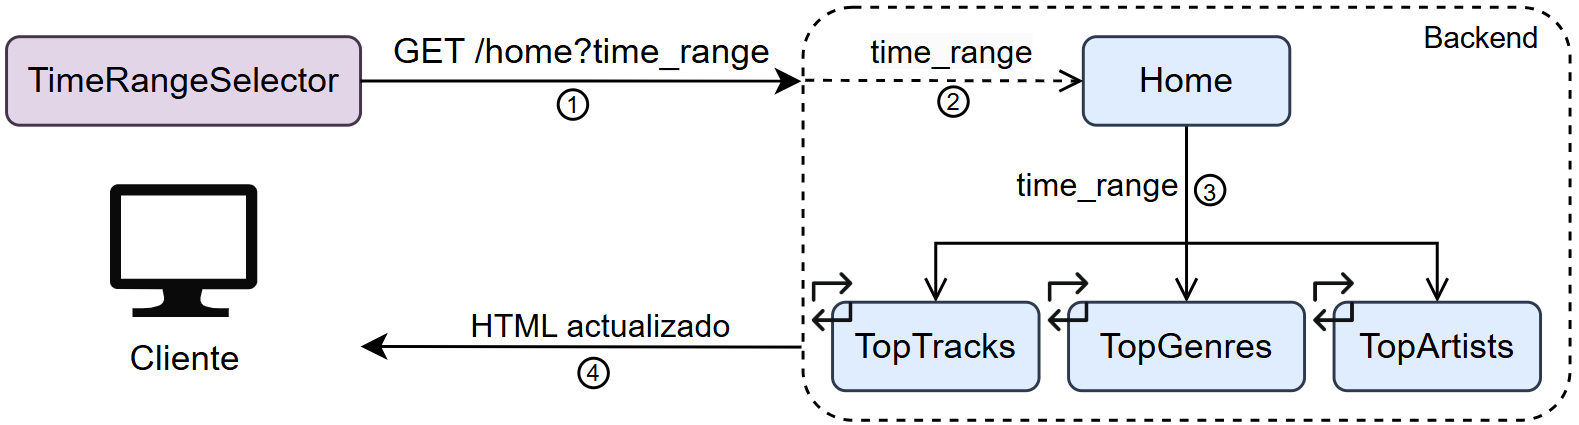
\includegraphics[width=0.8\textwidth]{figures/implementacion/actualizacion_tops.png}
    \vspace{10pt}
    \caption{Diagrama explicativo de la actualización de las estadísticas básicas del \textit{Home}.}
    \label{fig:actualizacion_tops}
\end{figure}

El componente \textbf{RecentlyPlayed} funciona de manera diferente, ya que no se ve afectado por el selector de tiempo. Al ser un componente de cliente, no puede acceder a las cookies directamente. En su lugar, utiliza el \texttt{useFetch} para obtener los datos desde el backend. Este componente también gestiona su propio estado para alternar entre mostrar las últimas 10 o 50 canciones reproducidas.

\subsection{Estadísticas Avanzadas (Stats)}

Las estadísticas avanzadas se encuentran en la página \texttt{/stats}, la cual está compuesta completamente por \textbf{componentes de cliente}. Debido a su mayor complejidad y carga de procesamiento, estas estadísticas se \textbf{cargan dinámicamente}, evitando que se envíen todas al navegador desde el inicio y mejorando el rendimiento.

\subsection*{Paso de Información entre Componentes del Cliente}

El componente \textbf{Stats} contiene la estructura principal de la página, incluyendo el \textbf{StatsGrid} (que muestra las tarjetas de estadísticas) y el \textbf{StatWrapper} (que gestiona la visualización de la estadística seleccionada). La gestión de los estados se centraliza en el componente padre \textbf{Stats}, mientras que, a través de \textit{props}, se pasa a los componentes hijos las funciones definidas que habilitan la actualización de esos estados (ver código en el anexo, algoritmo \ref{alg:stats_component}).

Cuando un \textbf{StatCard} es clicada, ejecuta dicha función y actualiza el estado \texttt{activeStat} con el valor del \texttt{statId} que contiene cada tarjeta y el estado \texttt{isModalOpen}, indicando que que se abra la ventana modal. Al detectar un cambio en su estado, \textbf{Stats} se vuelve a renderizar, provocando, a su vez, el renderizado de sus componentes hijos. Ahora, \textbf{StatWrapper} obtiene el valor \texttt{activeStat} como un \textit{prop} y puede cargar la estadística apropiada.

\begin{figure}[H]
    \centering
    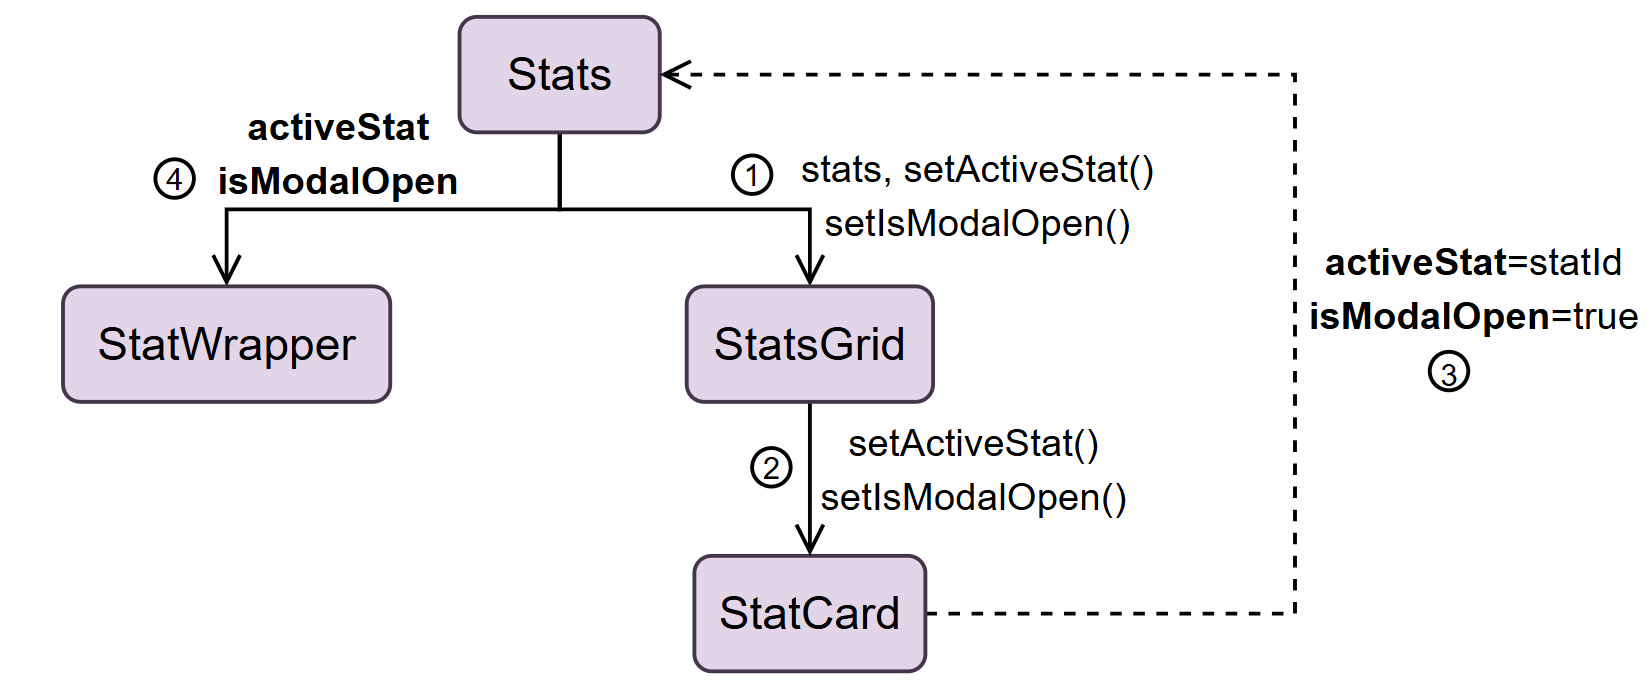
\includegraphics[width=0.7\textwidth]{figures/implementacion/actualizacion_stats.png}
    \vspace{10pt}
    \caption{Diagrama explicativo de la actualización de la página \textit{Stats} para detectar la selección de la estadística.}
    \label{fig:actualizacion_stats}
\end{figure}

Como se puede ver en la figura \ref{fig:actualizacion_stats}, los componentes \textbf{StatCard} y \textbf{StatWrapper} no se comunican directamente, \underline{si no que lo hacen de manera indirecta a través del componente} \underline{superior común \textbf{Stats}}. Esto es un flujo de datos típico entre componentes de cliente de \textit{React}.

\subsection*{Carga Dinámica de las Estadísticas}

Además del \texttt{statId}, \textbf{StatWrapper} recibe, mediante \textbf{props}, el estado de visibilidad del modal (\texttt{isModalOpen}) y una función de cierre (\texttt{handleCloseModal()}) que permite resetear el estado al cerrar la ventana. Para simplificar la gestión de la ventana modal, se ha utilizado la librería \textbf{Radix UI}, la cual no afecta el proceso de selección y carga de las estadísticas.

Dentro del componente \textbf{StatWrapper} existe un objeto que asocia cada \texttt{statId} con su respectivo componente (algoritmo \ref{alg:stat_components}). Mediante la función \textbf{dynamic()} de \textit{Next.js}, se realiza una carga dinámica en el momento en el que sea necesario renderizar el componente indicado. Cada vez que se selecciona una nueva estadística, se desmonta el componente anterior y se renderiza el nuevo en su lugar. También se elimina el componente cuando ya no sea necesario renderizarlo (al cerrar la ventana modal), por lo que el código relacionado con las estadísticas solo existe en el navegador el tiempo necesario, liberándolo de todo procesamiento innecesario.

Para más detalle del proceso de carga dinámico, se puede encontrar el código completo del componente \textbf{StatWrapper} en el anexo, algoritmo \ref{alg:stat_wrapper}.

\begin{ifalgorithm}[H]
    \begin{lstlisting}
    const statComponents = {
      "hall-of-fame": dynamic(() => import("@/components/stats/HallOfFame")),
      "estaciones-musicales": dynamic(() => import("@/components/stats/EstacionesMusicales")),
      "huella-del-dia": dynamic(() => import("@/components/stats/HuellaDelDia")),
      "la-bitacora": dynamic(() => import("@/components/stats/LaBitacora")),
      "tus-decadas": dynamic(() => import("@/components/stats/TusDecadas")),
      "indice-de-interferencia": dynamic(() => import("@/components/stats/IndiceDeInterferencia")),
    };

    const DynamicComponent = statComponents[statId as keyof typeof statComponents];
    \end{lstlisting}
    \caption{Carga dinámica de componentes de estadísticas utilizando \texttt{dynamic} de Next.js.}
    \label{alg:stat_components}
\end{ifalgorithm}

A continuación se detallarán algunos aspectos concretos de la implementación de cada estadística. Para mantener la redacción compacta, no se va a dar una descripción exhaustiva de todas las funcionalidades, si no que se centrará solamente en aquellos puntos notables o partes que requieran una mención especial. Tampoco se explicarán los aspectos de la gestión de errores o de carga, ya que recaen más en el ámbito de las \nameref{sec:optimizaciones} y todas lo hacen de manera muy similar.

Para cada estadística, se ha usado el sistema de renderizado de gráficos más conveniente y óptimo para la situación. En la siguiente tabla \ref{tab:librerias_renderizado} se recogen dichas librerías:

\begin{table}[htbp]
    \centering
    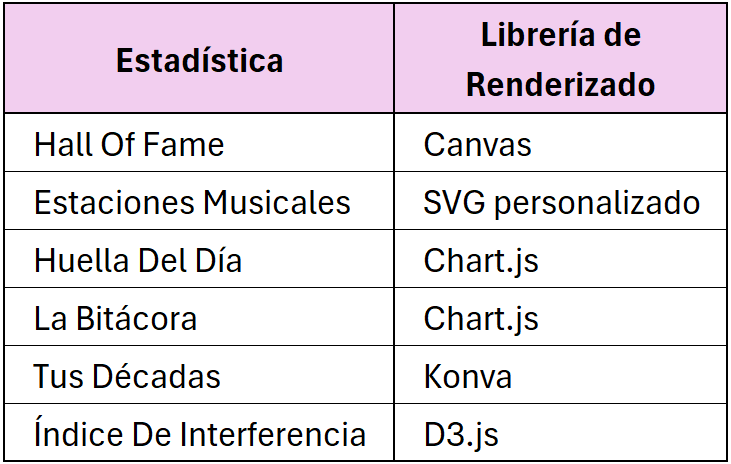
\includegraphics[width=0.5\textwidth]{figures/implementacion/librerias_renderizado.png}
    \captionsetup{skip=5pt}
    \caption{Librerías de renderizado seleccionadas para cada estadística avanzada.}
    \label{tab:librerias_renderizado}
\end{table}

\subsubsection*{i. Hall Of Fame}

La estadística \textit{Hall Of Fame} permite al usuario visualizar una cuadrícula con los álbumes más representativos de su historial de reproducción. Para su renderizado, se emplea el componente \textbf{Image} de \textit{Next.js}, que optimiza la carga y presentación de las imágenes de manera automática. Además, se ha implementado un sistema de generación de imagen que permite capturar la cuadrícula generado en \textbf{canvas} mediante la librería \textbf{html2canvas}.

\newpage

Antes de enviar la imagen al backend, la imagen se somete a un proceso de optimización (función \texttt{optimizeImage()} en el algoritmo \ref{alg:optimize_image}) para reducir su tamaño y que ocupe el límite máximo de datos a enviar (256 KB) con la máxima calidad posible bajo dicha restricción.

\subsubsection*{ii. Estaciones Musicales}

La estadística \textit{Estaciones Musicales} muestra la relación entre las estaciones del año y los hábitos de escucha del usuario mediante un gráfico de tipo ``donut'', donde cada estación se representa con un color distintivo y un icono característico.

La interfaz es interactiva y responde a los movimientos del cursor. Al pasar sobre una estación, el segmento correspondiente se resalta con una animación de expansión, y se despliega una tarjeta emergente con información sobre el artista y género más representativos de ese periodo. La posición del \textit{tooltip} se ajusta dinámicamente en función de la ubicación del cursor. La creación de estos segmentos y la gestión de las animaciones se realiza de forma manual mediante SVGs personalizados con la función en el algoritmo \ref{alg:calculate_path}.

\subsubsection*{iii. Huella Del Día}

La estadística \textit{Huella del Día} muestra la distribución de los minutos de escucha a lo largo del día mediante un gráfico de líneas, permitiendo al usuario identificar sus horas de mayor consumo musical. Para su implementación, la librería \texttt{react-chartjs-2} ayuda con la integración de \textbf{chart.js} en un entorno \textit{React}.

El gráfico cuenta con dos elementos:
\begin{itemize}
    \item \textbf{Línea principal}: Representa la cantidad de minutos de reproducción en cada hora del día.
    \item \textbf{Punto destacado}: Resalta la hora con mayor actividad, facilitando su identificación visual.
\end{itemize}

Además, se incluye un mensaje dinámico que indica al usuario su hora de mayor escucha, resaltando este dato con un color distintivo para mejorar su visibilidad.

\subsubsection*{iv. La Bitácora}

La estadística \textit{La Bitácora} permite visualizar la evolución de las canciones guardadas por el usuario a lo largo del tiempo mediante un gráfico de barras interactivo que permite navegar entre distintos niveles de granularidad: \textbf{años}, \textbf{meses} y \textbf{días}.

Para su implementación, se ha utilizado la biblioteca \textbf{chart.js} integrada también con \texttt{react-chartjs-2}.

\subsubsection*{v. Tus Décadas}

La estadística \textit{Tus Décadas} permite visualizar la distribución de las canciones guardadas por el usuario a lo largo de diferentes décadas mediante una línea de tiempo interactiva que organiza las portadas de los álbumes por año, agrupándolos en bloques de diez años. Al igual que la estadística anterior, para integrar la biblioteca \textbf{Konva} en un entorno \textit{React}, se ha utilizado la biblioteca \texttt{react-konva}.

El sistema incorpora las siguientes opciones de interacción con la gráfica:
\begin{itemize}
    \item \textbf{Navegación mediante desplazamiento}: Permite moverse horizontal y verticalmente a lo largo de la línea de tiempo para explorar los álbumes de cada década. Esto se gestiona con el componente \texttt{Stage} de \textit{Konva}, como se muestra en el algoritmo \ref{alg:stage_tus_decadas}
    \item \textbf{Zoom dinámico}: Se ha implementado un sistema de \textit{zoom} con la rueda del ratón, facilitando la exploración de los datos en distintos niveles de detalle. La función encargada se puede encontrar en el algoritmo \ref{alg:handle_wheel_tus_decadas}.
\end{itemize}

\subsubsection*{vi. Índice De Interferencia}

La estadística \textit{Índice de Interferencia}, la más abstracta de todas, representa la diferencia entre los hábitos de escucha del usuario y su comportamiento actual mediante una visualización basada en ondas sinusoidales. Los datos de base corresponden a la \textbf{media de la popularidad} de las canciones que el usuario suele escuchar, determinada a partir de su biblioteca de canciones guardadas, y la popularidad de lo que está escuchando en el momento, calculada a partir de sus últimas 50 reproducciones. Estos valores de popularidad, que son numéricos, se traducen a la frecuencia de cada onda representada en la visualización.

Para su implementación, se ha utilizado la biblioteca \textbf{D3.js}, más capaz que \textit{chart.js}, y que facilita la generación de gráficos SVG optimizados. Los datos de frecuencia se obtienen desde el backend y se interpolan (algoritmo \ref{alg:generate_wave_data}) para construir las ondas representadas en la visualización (algoritmo \ref{alg:draw_wave}).

El sistema permite visualizar las siguientes ondas:
\begin{itemize}
    \item \textbf{Frecuencia habitual}: Representa el patrón de escucha estándar del usuario.
    \item \textbf{Frecuencia del momento}: Refleja la frecuencia de escucha actual.
    \item \textbf{Onda combinada}: Muestra la interferencia entre ambas frecuencias, resaltando las diferencias entre el comportamiento habitual y el actual.
\end{itemize}

El cálculo de la interferencia entre las dos ondas originales se hace mediante la suma los respectivos puntos en cada una. Esto se realiza con la siguiente función sencilla que se muestra en el algoritmo \ref{alg:combined_wave}, que genera los datos para la función de dibujado de onda:

\begin{ifalgorithm}[H]
    \begin{lstlisting}
    const combinedData = normalData.map((d, i) => ({
        x: d.x,
        y: d.y + actualData[i].y,
    }));
    \end{lstlisting}
    \caption{Cálculo de la onda combinada en \textit{Índice de Interferencia} sumando las ondas de la frecuencia habitual y la frecuencia actual.}
    \label{alg:combined_wave}
\end{ifalgorithm}

\newpage

\section{Implementación del Backend}

El backend de la aplicación se encarga de gestionar la comunicación con la API de \textit{Spotify}, procesar los datos recibidos y servir la información al frontend de manera eficiente. A continuación, se detallan los aspectos más relevantes de su implementación, incluyendo la lógica aplicada en el tratamiento de datos (en forma de pseudocódigo, para facilitar la compresión) y las estructuras de datos definidas para el fácil consumo del frontend.

Para evitar la sobrecarga del contenido principal, todo el contenido se encuentra en el \hyperref[ch:anexoD]{Anexo D}. Mediante esta lista, se podrá acceder a los contenidos concretos, agrupados por estadística:

\begin{itemize}
    \item \textbf{Hall Of Fame}: \ref{sec:backend_hall_of_fame}
    \item \textbf{Estaciones Musicales}: \ref{sec:backend_estaciones_musicales}
    \item \textbf{Huella Del Día}: \ref{sec:backend_huella_del_dia}
    \item \textbf{La Bitácora}: \ref{sec:backend_la_bitacora}
    \item \textbf{Tus Décadas}: \ref{sec:backend_tus_decadas}
    \item \textbf{Índice De Interferencia}: \ref{sec:backend_indice_de_interferencia}
\end{itemize}

\section{Middleware}

El \textit{middleware} en \textit{Next.js} permite interceptar y modificar las solicitudes HTTP antes de que lleguen a las rutas del \textit{App Router} o los endpoints de los \textit{Route Handers}. En esta aplicación, se usa como un sistema de separación entre las rutas para usuarios no autenticados (\texttt{/}, la raíz) y las rutas protegidas tras las autenticación y autorización (\texttt{/home} y \texttt{/stats}). Su código completo se encuentra disponible en el anexo, en el algoritmo \ref{alg:middleware}.

\subsection{Funcionamiento del Middleware}

El \textit{middleware} se aplica de manera global a las rutas \texttt{/home}, \texttt{/stats} y sus subrutas, ejecutándose antes de que las peticiones alcancen el backend. Su función principal es \textbf{verificar si el usuario está autenticado y autorizad}o para acceder a estas secciones protegidas. Para ello, realiza una comprobación de la existencia de las cookies de autenticación: el \texttt{access\_token} y el \texttt{refresh\_token}. Si ambas están presentes, la solicitud se considera válida y se permite el acceso a la página correspondiente.

Dado que el \texttt{access\_token} tiene una validez limitada de una hora, el \textit{middleware} también se encarga de \textbf{gestionar su renovación automática} cuando expira. En caso de no detectar un \texttt{access\_token} pero sí un \texttt{refresh\_token} válido, se invoca la función \texttt{renovarAccessToken()} (algoritmo \ref{alg:renovar_access_token}), la cual interactúa con la API de \textit{Spotify} utilizando las credenciales de la aplicación (\textit{Client ID} y \textit{Client Secret}) para solicitar un nuevo token de acceso. Como el \textit{middleware} se ejecuta en el servidor, el acceso a estas credenciales es seguro, ya que nunca son expuestas en el cliente. Esta estrategia permite extender la sesión del usuario sin requerir una nueva autenticación manual, mejorando la experiencia de usuario.

En la siguiente tabla \ref{tab:middleware_opciones} se han resumido todas las posibilidades y las acciones respectivas que el \textit{middleware} llevaría a cabo:

\begin{table}[htbp]
    \centering
    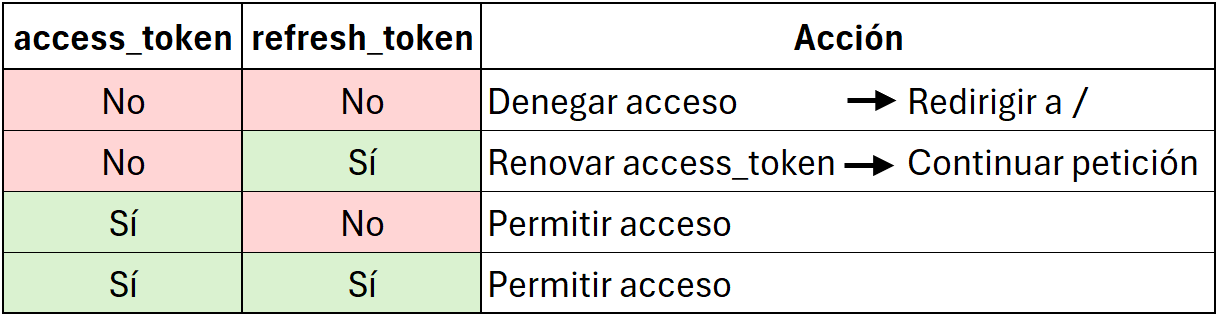
\includegraphics[width=0.75\textwidth]{figures/implementacion/middleware_opciones.png}
    \captionsetup{skip=10pt}
    \caption{Acciones del \textit{middleware} en todos los casos posibles de existencia de tokens.}
    \label{tab:middleware_opciones}
\end{table}

\subsection{Limitaciones y Consideraciones de Seguridad}

Si bien el sistema de autenticación definido es funcional y práctico para este tipo de aplicación, existe una vulnerabilidad potencial: el \textit{middleware} solo verifica la existencia de los tokens, \textbf{pero no su validez}. Esto significa que un usuario malintencionado podría crear manualmente cookies con los nombres \texttt{access\_token} y \texttt{refresh\_token} y valores aleatorios, lo que le permitiría acceder a la interfaz protegida. No obstante, cualquier intento de obtener datos desde la API de \textit{Spotify} fallaría, ya que los tokens falsificados no serían reconocidos por el servicio.

Para mitigar esta vulnerabilidad, se podría implementar una validación adicional enviando una solicitud a la API desde el \textit{middleware} para comprobar si el token es válido antes de conceder acceso. Sin embargo, esta solución implicaría una llamada extra a \textit{Spotify} en cada solicitud, lo que aumentaría la carga en la API y afectaría el tiempo de carga de la aplicación. Dado que la probabilidad de explotación de esta vulnerabilidad es baja en el contexto de este proyecto, \textbf{se ha decidido no implementar esta verificación adicional} para evitar un consumo innecesario de recursos.


\section{Optimizaciones} \label{sec:optimizaciones}
De todas las estadísticas:
los aspectos de la gestión de errores o de carga

En La Bitácora:
Para mejorar la experiencia de usuario y la eficiencia del sistema, se han implementado las siguientes optimizaciones:
\begin{itemize}
    \item \textbf{Ordenación de datos}: Los valores se ordenan cronológicamente para facilitar su interpretación.
    \item \textbf{Formateo de etiquetas}: Se han personalizado los nombres de los meses y días para mejorar la legibilidad.
    \item \textbf{Evitación de recargas innecesarias}: Se han optimizado las llamadas a la API para evitar periodos de carga entre clics, haciendo la navegación más fluida.
    \item \textbf{Cálculo dinámico de porcentajes}: Se muestra en los \textit{tooltips} de cada barra el porcentaje que representa cada período sobre el total.
\end{itemize}

Para Indice de Interferencia:
Para mejorar la experiencia del usuario, se han implementado diversas optimizaciones:
\begin{itemize}
    \item \textbf{Transiciones suaves}: Se han añadido animaciones progresivas en la aparición de las ondas para mejorar la fluidez visual.
    \item \textbf{Efectos de resaltado}: Se han aplicado filtros de \texttt{drop-shadow} dinámicos para destacar la onda seleccionada.
    \item \textbf{Interactividad mejorada}: Se permite alternar entre la vista de ondas individuales y la onda combinada mediante un botón, facilitando el análisis de la interferencia entre ambas frecuencias.
\end{itemize}

Para Tus Décadas:
Para mejorar la experiencia del usuario y la eficiencia del sistema, se han aplicado las siguientes optimizaciones:
\begin{itemize}
    \item \textbf{Ajuste dinámico del lienzo}: Se detecta automáticamente el tamaño de la pantalla del usuario para adaptar la visualización de la línea de tiempo, utilizando el \textit{hook} \texttt{useRef}.
    \item \textbf{Renderización optimizada}: Se emplean capas (\textit{layers}) dentro de \texttt{react-konva} para procesar solo los elementos visibles, mejorando el rendimiento en dispositivos con menor capacidad gráfica.
\end{itemize}


